\section{Vypracování}
\subsection{Generalizace budov}

Generalizace budov do úrovně detailu LOD0 (Level of Detail 0) patří mezi základní úlohy digitální kartografie a geografických informačních systémů. V praxi se s ní setkáváme při zjednodušování rozsáhlých datových sad (např. ZABAGED) pro přehlednější vizualizaci v menších měřítkách.
Cílem je pro daný polygon budovy $B = \{p_1, \dots, p_n\}$ efektivně nalézt reprezentativní obdélník $G(B)$, který zachovává její hlavní směry a celkovou rozlohu. 

Zatímco ruční generalizace by byla pro tisíce budov časově neúnosná, automatizované algoritmy využívají geometrické a statistické metody k nalezení dominantního směru polygonu $\sigma$. Společným rysem všech implementovaných metod je finální vytvoření opsaného obdélníku a jeho přeškálování tak, aby odpovídal rozloze původní budovy. 
Škálovací koeficient $k$ je dán poměrem ploch:
\[
  k = \frac{A_b}{A_m}
\]
kde $A_b$ je plocha původní budovy a $A_m$ je plocha neškálovaného obdélníku. Všechny vektory od těžiště k vrcholům obdélníku jsou následně přenásobeny hodnotou $\sqrt{k}$.


\subsection{Konstrukce konvexní obálky - Jarvis Scan}

Konvexní obálka (Convex Hull) množiny bodů $P$ je nejmenší konvexní polygon, který obsahuje všechny body z $P$. Slouží jako nezbytný vstup pro další geometrické operace, zejména pro vyhledání minimálního opsaného obdélníku. V této aplikaci byl pro její konstrukci implementován algoritmus Jarvis Scan (známý jako balení dárku).

Algoritmus iterativně hledá body ležící na hranici obálky. Výchozím bodem (pivotem) $q$ je bod s minimální souřadnicí $y$. Následně se v každém kroku hledá z množiny zbývajících bodů takový bod $p_i$, který s aktuálním směrem obálky svírá největší vnitřní úhel $\omega$. Algoritmus končí ve chvíli, kdy se jako další bod na obálce vybere opět výchozí pivot $q$.
\newpage

\textbf{Pseudokód Jarvis Scan}
\begin{algorithm}[H]
\caption{Jarvis Scan ($P = \{p_1, \dots, p_n\}$)}
\label{alg:jarvis}
\begin{algorithmic}[1]
\State Najdi bod $q \in P$ s minimální souřadnicí $y$
\State Inicializuj obálku $CH = \{q\}$
\State $p_{curr} = q$
\State Definuj pomocný bod $p_{prev} = (x_q - 1, y_q)$ \Comment{Pro počáteční vektor}
\Repeat
    \State $\omega_{max} = 0$, $p_{next} = \text{null}$
    \For{každý bod $p_i \in P, p_i \neq p_{curr}$}
        \State Spočítej úhel $\omega$ mezi vektory $(p_{curr} - p_{prev})$ a $(p_i - p_{curr})$
        \If{$\omega > \omega_{max}$}
            \State $\omega_{max} = \omega$
            \State $p_{next} = p_i$
        \EndIf
    \EndFor
    \State Přidej $p_{next}$ do $CH$
    \State $p_{prev} = p_{curr}$
    \State $p_{curr} = p_{next}$
\Until{$p_{curr} == q$}
\State \Return $CH$
\end{algorithmic}
\end{algorithm}



\subsection{Graham Scan}
Graham Scan je další z mnoha metod pro vytvoření konvexní obálky. 
Algoritmus začíná tím, že najde bod, který má nejmenší souřadnici Y. Bude sloužit jako náš počáteční bod, tzv. pivot.
Všechny ostatní body se vezmou a seřadí se podle toho, jaký úhel svírají s horizontální osou procházející pivotem.
Nyní se vyfiltrují přebytečné body.
Pokud více bodů leží na jedné přímce (mají stejný úhel), zajímá nás pouze ten nejvzdálenější, všechny bližší se odstraní.
Nyní se vytvoří zásobník a pomocí cyklu while se prochází zbytek bodů.
Pro každý nový bod se vezmou poslední dva body ze zásobníku a zkotroluje se, zda jsou levotočivé či pravotočivé. Když jsou levotočivé, poslední bod je bodem konvexní obálky. Pokud jsou pravotočivé, poslední bod nemůže být bodem konvexní obálky. 

\newpage
\textbf{Pseudokód Graham Scan}
\begin{algorithm}[H]
\caption{Graham Scan (P)}
\label{alg:graham}
\begin{algorithmic}[1]
    \If{$|P| < 3$}
        \State \Return $P$ \Comment{Ošetření malého počtu bodů}
    \EndIf
    
    \State $q \gets \text{bod z } P \text{ s min. } Y \text{)}$
    \State $Body \gets P \setminus \{q\}$
    
    \State Seřaď $Body$ vzestupně podle  úhlu vůči $q$
    \
    
    \State $FiltrovaneBody \gets \text{prázdný seznam}$
    \For{$i \gets 0 \textbf{ to } |Body| - 1$}
        \If{$i < |Body| - 1 \textbf{ and } \text{úhel}(Body[i]) = \text{úhel}(Body[i+1])$}
            \State \textbf{continue} \Comment{Ignoruj bližší kolineární body}
        \EndIf
        \State $FiltrovaneBody.\text{append}(Body[i])$
    \EndFor
    
    \If{$|FiltrovaneBody| < 2$}
        \State \Return $q \cup FiltrovaneBody$
    \EndIf
    
    \State $S \gets \text{prázdný zásobník}$
    \State $S.\text{push}(q)$
    \State $S.\text{push}(FiltrovaneBody[0])$
    
    \For{$i \gets 1 \textbf{ to } |FiltrovaneBody| - 1$}
        \State $NovyBod \gets FiltrovaneBody[i]$
        \While{$|S| > 1 \textbf{ and } \text{Orientace}(S[-2], S[-1], NovyBod) \le 0$}
            \State $S.\text{pop}()$ \Comment{Odstraňuj při pravotočivé zatáčce}
        \EndWhile
        \State $S.\text{push}(NovyBod)$
    \EndFor
    
    \State \Return $S$
\end{algorithmic}
\end{algorithm}
\subsection{Minimum Area Enclosing Rectangle}

Metoda Minimum Area Enclosing Rectangle (MAER/MBR) vyhledává ohraničující obdélník s absolutně nejmenší plochou. Algoritmus pracuje nad konvexní obálkou polygonu. Využívá principu, že minimální opsaný obdélník sdílí alespoň jednu stranu s hranou konvexní obálky. 

Pro každou hranu určí její směrový úhel $\sigma$ a celou konvexní obálku o tento úhel zpětně orotuje. Následně se pro orotovanou obálku spočítá min-max box (pravoúhlý hraniční obdélník) a jeho plocha. Výsledkem algoritmu je orotovaný obdélník, u kterého byla nalezena nejmenší plocha. Ten je pak v hlavní funkci generalizace přeškálován.
\\[2mm]

\textbf{Pseudokód MAER}
\begin{algorithm}[H]
\caption{Minimum Area Enclosing Rectangle ($B$)}
\label{alg:MAER}
\begin{algorithmic}[1]
\State $CH = \text{JarvisScan}(B)$
\State $A_{min} = \infty$, $MBR = \text{null}$, $\sigma_{min} = 0$
\For{každou hranu $e_i(p_i, p_{i+1}) \in CH$}
    \State $\sigma_i = \arctan2(y_{i+1} - y_i, x_{i+1} - x_i)$
    \State $CH_{rot} = \text{Rotate}(CH, -\sigma_i)$
    \State $MMB = \text{CreateMinMaxBox}(CH_{rot})$
    \State $A_i = \text{Area}(MMB)$
    \If{$A_i < A_{min}$}
        \State $A_{min} = A_i$
        \State $\sigma_{min} = \sigma_i$
        \State $MBR = MMB$
    \EndIf
\EndFor
\State $MBR_{res} = \text{Rotate}(MBR, \sigma_{min})$
\State \Return $\text{ResizeRectangle}(MBR_{res}, \text{Area}(B))$
\end{algorithmic}
\end{algorithm}




\subsection{PCA (Principal Component Analysis)}

Analýza hlavních komponent (PCA) je statistická metoda, která hledá směry největšího rozptylu dat. V kartografii se lomové body budovy interpretují jako množina bodů v rovině, z jejichž souřadnic se vytvoří matice a následně kovarianční matice $C$.

Výpočtem vlastních čísel a vlastních vektorů této matice (např. metodou SVD, Singular Value Decomposition) získáme hlavní osu budovy. Směrový úhel $\sigma$ je určen vlastním vektorem $\vec{v}$, který náleží největšímu vlastnímu číslu.

\newpage
\textbf{Pseudokód PCA}
\begin{algorithm}[H]
\caption{PCA ($B = \{p_1, \dots, p_n\}$)}
\label{alg:PCA}
\begin{algorithmic}[1]
\State Extrahuj vektory souřadnic $X = \{x_1, \dots, x_n\}$ a $Y = \{y_1, \dots, y_n\}$
\State Vytvoř matici $A = [X, Y]$
\State Spočítej kovarianční matici $C = \text{cov}(A)$
\State Proved SVD rozklad matice $C \rightarrow [U, S, V]$
\State Získej dominantní vektor $\vec{v} = V_0$
\State $\sigma = \arctan2(v_y, v_x)$
\State $B_{rot} = \text{Rotate}(B, -\sigma)$
\State $MMB = \text{CreateMinMaxBox}(B_{rot})$
\State $MBR = \text{Rotate}(MMB, \sigma)$
\State \Return $\text{ResizeRectangle}(MBR, \text{Area}(B))$
\end{algorithmic}
\end{algorithm}





\subsection{Longest Edge}

Metoda nejdelší hrany představuje nejjednodušší a výpočetně nejméně náročný přístup k určení dominantního směru. Algoritmus prochází všechny hrany polygonu budovy a pomocí Pythagorovy věty vyhodnocuje jejich euklidovskou délku $s_i$. Předpokládá se, že nejdelší kompaktní stěna budovy nejlépe definuje její hlavní orientaci $\sigma$.

\textbf{Pseudokód Longest Edge}
\begin{algorithm}[H]
\caption{Longest Edge ($B$)}
\label{alg:longestedge}
\begin{algorithmic}[1]
\State $s_{max} = 0$, $\sigma_{max} = 0$
\For{každou hranu $e_i(p_i, p_{i+1}) \in B$}
    \State $s_i = \sqrt{(x_{i+1} - x_i)^2 + (y_{i+1} - y_i)^2}$
    \If{$s_i > s_{max}$}
        \State $s_{max} = s_i$
        \State $\sigma_{max} = \arctan2(y_{i+1} - y_i, x_{i+1} - x_i)$
    \EndIf
\EndFor
\State $B_{rot} = \text{Rotate}(B, -\sigma_{max})$
\State $MMB = \text{CreateMinMaxBox}(B_{rot})$
\State $MBR = \text{Rotate}(MMB, \sigma_{max})$
\State \Return $\text{ResizeRectangle}(MBR, \text{Area}(B))$
\end{algorithmic}
\end{algorithm}




\subsection{Wall Average}
Wall Average předpokládá, že většina budov má pravoúhlý půdorys. Je to robustní metoda, ale citlivá na „nepravé“ úhly.
Algoritmus prochází všechny hrany budovy a zjišťuje, jak moc se odchylují od pravého úhlu.
Prvním krokem je určení směrnic $\sigma_i$ pro všechny hrany budovy. Následně se pro každý vrchol $p_i$ spočte relativní úhel $\omega_i$ mezi hranami: 
\[
\omega_i= | \sigma_{i, i+1} - \sigma_{i-1, i}|.
\]
Následně se vypočte násobek pravého úhlu, tedy kolikrát se do daného úhlu $\omega_i$ vleze pravý úhel ($k_i$).
Vypočteme koeficient $k_i$:
\[
k_i = \frac{2\omega_i}{\pi}.
\]
Dále je potřeba zjistit, jaká je odchylka hrany od nejbližšího pravého úhlu. Vypočte se tzv. orientovaný zbytek $r_i$:
\[
r_i = (k_i -\text{round}(k_i))\cdot\frac{\pi}{2}.
\]
Konečný hlavní směr budovy $\sigma$ se vypočítá tak, že vezmeme základní směr a přičteme k němu vážený průměr všech zjištěných odchylek $r_i$. Váhou v tomto výpočtu je délka dané hrany $s_i$. Tím se zajistí, že dlouhé stěny ovlivní výsledek mnohem více než krátké výklenky.
\[
\sigma = \sigma_{1} + \frac{\sum^n_{i=1} r_i\cdot s_i}{\sum^n_{i=1} s_i}
\]

\newpage
\textbf{Pseudokód Wall Average}
\begin{algorithm}
\caption{Wall Average}
\label{alg:wallaverage}
\begin{algorithmic}[1]
    \State $n \gets |B|$
    \State $sum\_rs \gets 0$
    \State $sum\_s \gets 0$
    
    \State $\sigma_1 \gets \text{atan2}(p_1.y - p_0.y, p_1.x - p_0.x)$ \Comment{Směrnice první hrany}
    
    \For{$i \gets 0 \textbf{ to } n - 1$}
        \State $p_1 \gets B[i]$
        \State $p_2 \gets B[(i+1) \bmod n]$
        
        \State $\Delta x \gets p_2.x - p_1.x$
        \State $\Delta y \gets p_2.y - p_1.y$
        
        \State $s_i \gets \sqrt{\Delta x^2 + \Delta y^2}$ \Comment{Délka hrany}
        \State $\sigma_i \gets \text{atan2}(\Delta y, \Delta x)$ \Comment{Směrnice hrany}
        
        \State $\omega_i \gets \sigma_i - \sigma_1$
        
        \State $k_i \gets \frac{2 \cdot \omega_i}{\pi}$ 
        \State $r_i \gets (k_i - \text{round}(k_i)) \cdot \frac{\pi}{2}$ 
        
        \State $sum\_rs \gets sum\_rs + (r_i \cdot s_i)$ \Comment{Suma vážených odchylek}
        \State $sum\_s \gets sum\_s + s_i$ \Comment{Suma délek stěn}
    \EndFor
    
    \State $\sigma_{avg} \gets \sigma_1 + \left(\frac{sum\_rs}{sum\_s}\right)$ \Comment{Hlavní směr budovy}
    
    \State $B_{rot} \gets \text{RotatePolygon}(B, -\sigma_{avg})$ 
    \State $(MMB, area) \gets \text{CreateMMB}(B_{rot})$ 
    
    \State $MBR \gets \text{RotatePolygon}(MMB, \sigma_{avg})$ 
    \State $MBR_{res} \gets \text{ResizeRectangle}(B, MBR)$ 
    
    \State \Return $MBR_{res}$
\end{algorithmic}
\end{algorithm}

\newpage
\subsection{Weighted Bisector}
Metoda Weighted Bisector  je další přístup pro určení hlavního směru  budovy. 
Základní myšlenkou je, že hlavní orientaci a proporce budovy nejlépe vystihují její nejdelší úhlopříčky.
Algoritmus nejprve identifikuje všechny možné spojnice (úhlopříčky) mezi vrcholy polygonu. Z nich se následně vyberou dvě absolutně nejdelší úhlopříčky.
Pro tyto dvě vybrané nejdelší úhlopříčky se zjistí dva hlavní parametry - jejich délky ($s_1$ a $s_2$), jejich směrnice ($\sigma_1$ a $\sigma_2$).
Konečný hlavní směr budovy $\sigma$ tvoří osu úhlu mezi těmito dvěma úhlopříčkami.  Aby delší úhlopříčka měla na výsledek větší vliv, počítá se vážený průměr jejich směrnic, kde váhou je právě délka příslušné úhlopříčky.

\[
\sigma = \frac{s_1\cdot \sigma_1 +s_2\cdot \sigma_2}{s_1 + s_2}
\]


\textbf{Pseudokód Weighted Bisector}
\begin{algorithm}
\caption{Weighted Bisector}
\label{alg:weightedbisector}
\begin{algorithmic}[1]
\State $n \gets |B|$
    \State $Diagonaly \gets \text{prázdný seznam}$
    
    \For{$i \gets 0 \textbf{ to } n - 1$}
        \For{$j \gets i + 1 \textbf{ to } n - 1$}
            \State $p_1 \gets B[i]$
            \State $p_2 \gets B[j]$
            
            \State $\Delta x \gets p_2.x - p_1.x$
            \State $\Delta y \gets p_2.y - p_1.y$
            
            \State $delka \gets \sqrt{\Delta x^2 + \Delta y^2}$
            \State $\sigma \gets \text{atan2}(\Delta y, \Delta x)$
            
            \State $\sigma \gets \sigma \bmod \pi$ \Comment{Normalizace, diagonály jsou neorientované}
            
            \State $Diagonaly.\text{append}((delka, \sigma))$
        \EndFor
    \EndFor
    
    \State Seřaď $Diagonaly$ sestupně podle proměnné $delka$
    
    \State $(s_1, \sigma_1) \gets Diagonaly[0]$ \Comment{První nejdelší diagonála}
    \State $(s_2, \sigma_2) \gets Diagonaly[1]$ 
    
    \State $\sigma_{avg} \gets \frac{s_1 \cdot \sigma_1 + s_2 \cdot \sigma_2}{s_1 + s_2}$ \Comment{Výpočet váženého průměru úhlů}
    
    \State $B_{rot} \gets \text{RotatePolygon}(B, -\sigma_{avg})$
    \State $(MMB, area) \gets \text{CreateMMB}(B_{rot})$ 
    
    \State $MBR \gets \text{RotatePolygon}(MMB, \sigma_{avg})$ 
    \State $MBR_{res} \gets \text{ResizeRectangle}(B, MBR)$ 
    
    \State \Return $MBR_{res}$
\end{algorithmic}
\end{algorithm}


\subsection{Načtení dat ze .shp}
Načtení dat se provádí pomocí knihovny \textit{shapefile}. 
Z důvodů různých souřadnicových systémů (souřadnice obrazovky jsou jiné než souřadnice shapefilu) bylo potřeba shapefile přemapovat do souřadnic obrazovky. 
Z původních shapefile souřadnic byly spočítány minima a maxima x-ových a y-ových souřadnic.
Z těchto údajů pak byly spočítany rozměry. 
\begin{lstlisting}[language=Python, caption = Rozměry shapefile.]
   #Calculate the dimensions
        shp_width = glob_max_x - glob_min_x
        shp_height = glob_max_y - glob_min_y 
\end{lstlisting}
Ty poté byly vycentrovány na střed obrazovky, zároveň byl zvolen 5 \% okraj, aby se budovy nedotýkaly okrajů, bylo zvoleno i měřítko. 
Následně byly body tvořící původní polygony přemapovány do souřadnic obrazovky a tyto přemapované body vytvořily polygony, které jsou poté načítány v samotné aplikaci. 
\begin{lstlisting}[language=Python, caption = Přemapování souřadnic bodů/polygonů.]
    for points in raw_polygons:
            scaled_points = []
            for x, y in points:
                screen_x = (x - glob_min_x) * scale + x_offset
                screen_y = canvas_height - ((y - glob_min_y) * scale + y_offset)
                scaled_points.append(QPointF(screen_x, screen_y))

            self.__buildings.append(QPolygonF(scaled_points))
\end{lstlisting}

\subsection{Vstupní data}
Vstupními daty jsou shapefile soubory budov ZABAGED, které byly upraveny v GIS software. 


Výstupem je aplikace vyvtořená v rozhraní QT, která generalizuje nahraný shapefile budov pomocí metod Minimum Area Enclosing Rectangle, PCA, Longest Edge, Wall Average a Weighted Bisector a zobrazuje, jak generalizace vypadá.

\begin{figure}[h!]
    \centering
    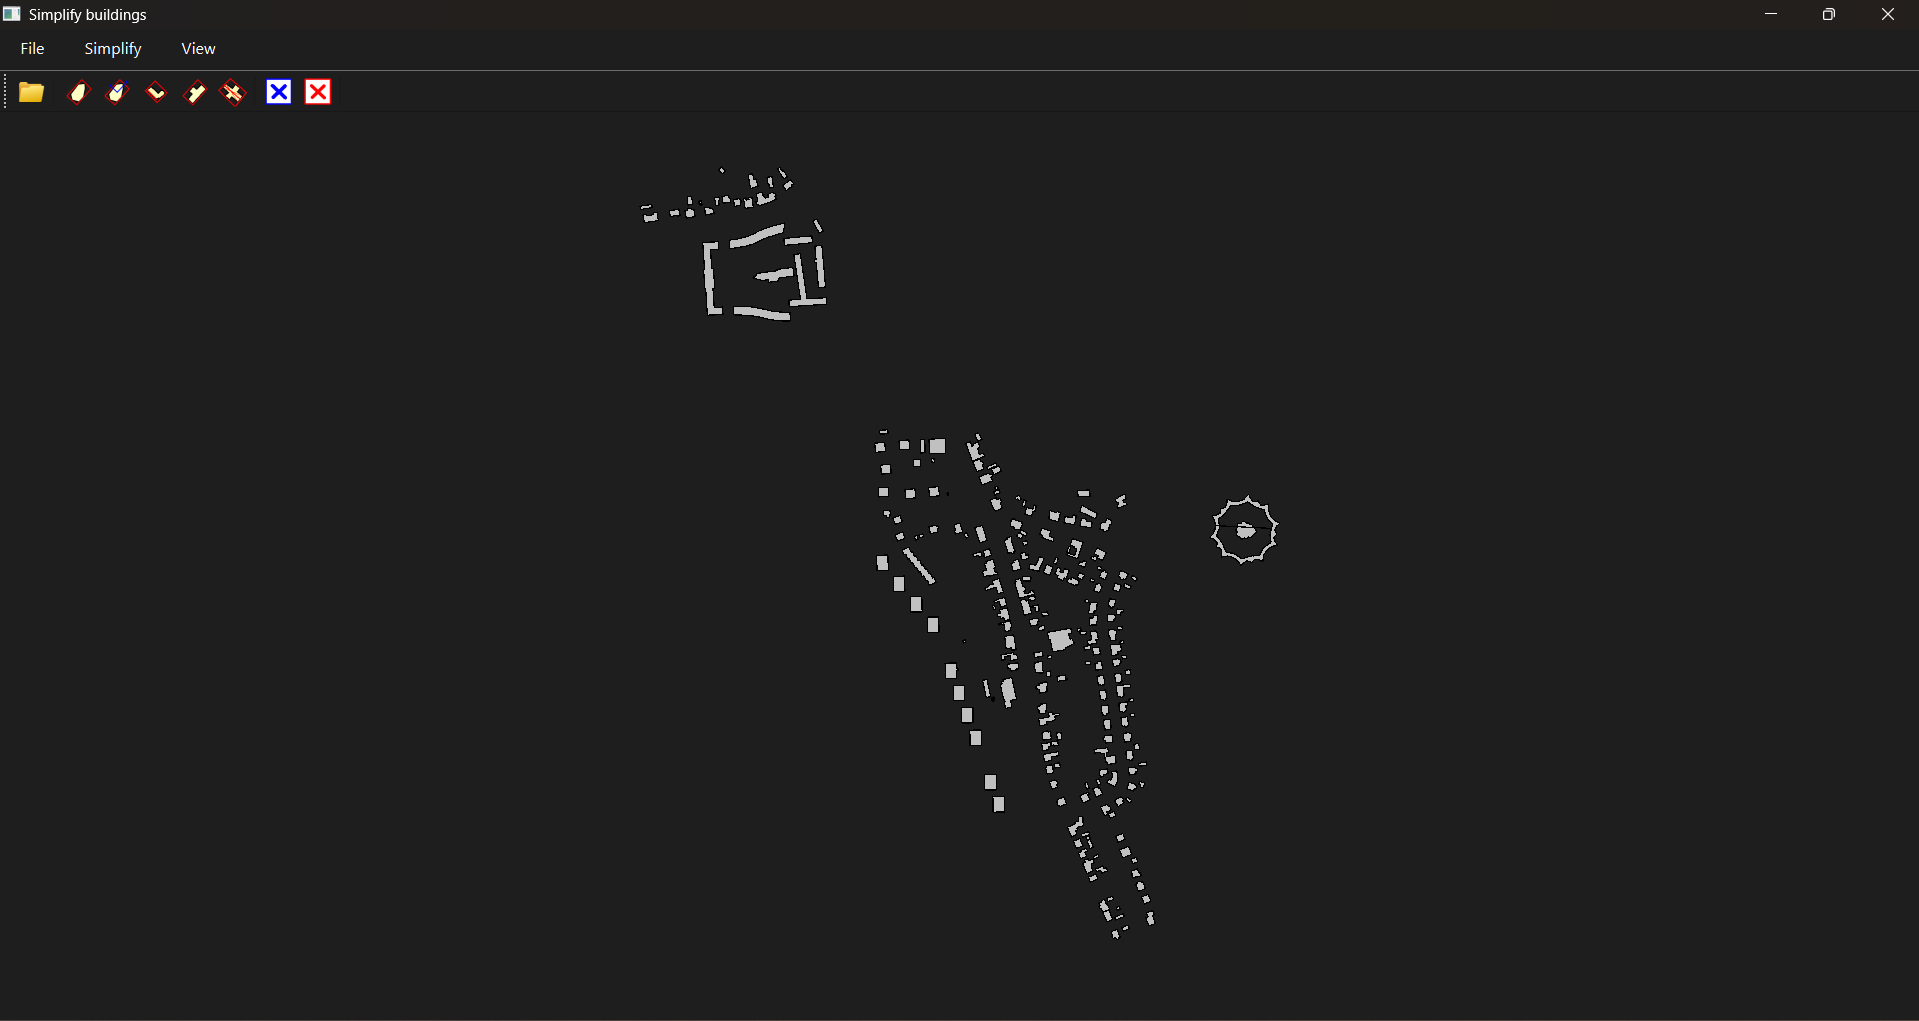
\includegraphics[width=0.9\linewidth]{figures/u2_screen.png}
    \caption{Printscreen vytvořené aplikace s načtenými daty.}
    \label{fig:obr1}
\end{figure}


\subsection{Dokumentace}
\subsubsection{Třída Algorithms}
Třída \textit{Algorithms} zahrnuje metody \textit{get2VectorsAngle} - vrátí úhel mezi dvěma vektory, \textit{getOrientation} - vrací orientaci (CW, CCW), \textit{getDistance} - vrací vzdálenost mezi dvěma body, \textit{createCHGraham} - vytvoří konvexní obálku pomocí Graham Scan, \textit{createCH} - vytvoří konvexní obálku pomocí Jarvis Scan, \textit{createMMB} - vytvoří minumum bounding box, \textit{rotatePolygon} - rotuje polygon zadaným úhlem, \textit{createMBR} - vytvoří minimum bounding rectangle, \textit{getArea} - vrátí rozlohu polygonu,
\textit{resizeRectangle} - přeškáluje polygon,\textit{simplifyBuildingMBR} - generalizuje polygon pomocí MBR, \textit{simplifyBuildingPCA}  - generalizuje polygon pomocí PCA, \textit{simplifyBuildingLongestEdge}  - generalizuje polygon pomocí Longest Edge, \textit{simplifyBuildingWallAverage}  - generalizuje polygon pomocí Wall Average a \textit{simplifyBuildingWeightedBisector}  - generalizuje polygon pomocí Weighted Bisector.



\subsubsection{Třída Draw}
Třída \textit{Draw} představuje stěžejní vizuální komponentu celé aplikace a slouží jako interaktivní kreslicí plátno (Canvas). Obsahuje metody pro zachytávání uživatelských vstupů, jako je \textit{mousePressEvent}, která umožňuje manuální zadávání lomových bodů polygonu pomocí myši. Samotné vykreslování veškeré grafiky zajišťuje metoda \textit{paintEvent}, která s využitím nástroje \textit{QPainter} vizuálně odlišuje původní budovy (šedě), konvexní obálky (modře) a výsledné generalizované obdélníky (červeně). 

Z hlediska datového toku obsahuje třída sadu přístupových metod. \textit{setMBR}, \textit{setMBRs} a \textit{setCH} slouží pro zápis vypočtených dat (výsledků algoritmů) zpět do plátna, zatímco \textit{getBuilding} a \textit{getBuildings} předávají data o polygonech zpět do výpočetního procesu. Klíčovou součástí třídy je metoda \textit{LoadShapesToScene}, která nejenže čte data z nahraného ESRI Shapefile, ale především zajišťuje nezbytnou transformaci, tedy výpočet měřítka, posun do středu plátna s ochranným okrajem a celkové přemapování globálních souřadnic do lokálního souřadnicového systému obrazovky. Třídu doplňuje metoda \textit{clearResults} pro vyčištění pracovní plochy.

\subsubsection{Třída Main Form}
Třída \textit{Main Form} plní roli řídicího softwarového uzlu (Controlleru), který spravuje grafické uživatelské rozhraní a spravuje rozložení okna včetně zapouzdřeného kreslicího plátna (\textit{Draw}). Její stěžejní funkcí je propojení vizuální části s výpočetní logikou prostřednictvím obsluhy událostí. Při interakci uživatele třída zprostředkuje tok dat: získá souřadnice budov z plátna, nechá třídu \textit{Algorithms} provést příslušnou generalizaci a vypočtené výsledky odešle zpět k překreslení scény. Třída tak řídí celou aplikaci a striktně odděluje uživatelské ovládání od geometrických výpočtů.

\newpage
\subsection{Výsledky a závěr}
V rámci této práce byla úspěšně vytvořena aplikace v prostředí PyQt6, která automatizuje proces generalizace půdorysů budov do úrovně detailu LOD0. Aplikace umožňuje bezproblémové načítání reálných datových sad ve formátu \textit{.shp} (např. ZABAGED) a jejich transformaci do souřadnicového systému obrazovky.

Pro určení dominantního směru budov bylo implementováno pět nezávislých algoritmů: Minimum Area Enclosing Rectangle (MAER), Principal Component Analysis (PCA), Longest Edge, Wall Average a Weighted Bisector. Součástí řešení je i robustní výpočet konvexní obálky s využitím algoritmů Jarvis Scan a časově efektivnějšího Graham Scan. Významným prvkem programu je ošetření singulárních případů (kolineární body, polygony s nulovou plochou), díky kterému aplikace nepadá ani na topologicky nekorektních datech. Všechny metody pak tedy zachovávají původní rozlohu budovy díky aplikovanému plošnému škálovacímu koeficientu $k$.

\subsubsection*{Porovnání metod a diskuze výsledků}

Při testování na reálných datech (zástavba historického centra, moderní sídliště, izolované rodinné domy) se ukázalo, že neexistuje jeden univerzálně nejlepší algoritmus. Každá metoda se hodí pro jiný typ zástavby i s ohledem na její rozložení:

\begin{itemize}
    \item \textbf{MAER / MBR} poskytuje vizuálně velmi stabilní obdélníky. Z principu své konstrukce však může u budov ve tvaru písmene "L", "U", nebo u diagonálně orientovaných bloků generovat neúměrně široké a zkreslené výsledky, které vizuálně nerespektují hmotu budovy.
    \begin{table}[h!]
\centering
\begin{tabular}{|c|c|c|}
\hline
 Izolovaná zástavba & Sídliště & Historické centrum  \\
 \hline
208/218 & 105/106  &  143/163 \\
\hline
 95,4 \% & 99,1\%  & 87,7\%  \\
 \hline
\end{tabular}
    \caption{Výsledky pro MAER / MBR.}
\label{table:MBR}
\end{table}

    \item \textbf{PCA} je výpočetně velmi rychlá metoda, která se hodí především na protáhlé liniové budovy a sídlištní zástavbu. Ukázala se však jako náchylná na drobné a asymetrické výstupky z jinak pravoúhlého půdorysu, které dokážou hlavní osu nechtěně vychýlit.
        \begin{table}[h!]
\centering
\begin{tabular}{|c|c|c|}
\hline
 Izolovaná zástavba & Sídliště & Historické centrum  \\
 \hline
88/218 & 73/106  &  64/163 \\
\hline
 40,4 \% & 68,9\%  & 39,3\%  \\
 \hline
\end{tabular}
    \caption{Výsledky pro PCA.}
\end{table}

    \item \textbf{Longest Edge} funguje spolehlivě u jednoduché izolované zástavby bez složitých detailů. Výrazně ale selhává u složitějších tvarů (např. historická zástavba), kde náhodná nejdelší kompaktní stěna nemusí vůbec reprezentovat reálnou orientaci celé budovy.
        \begin{table}[h!]
\centering
\begin{tabular}{|c|c|c|}
\hline
 Izolovaná zástavba & Sídliště & Historické centrum  \\
 \hline
213/218 & 106/106  &  144/163 \\
\hline
 97,7 \% & 100\%  & 88,3\%  \\
 \hline
\end{tabular}
    \caption{Výsledky pro Longest Edge.}
\end{table}

    \item \textbf{Wall Average} se ukázal jako mimořádně robustní algoritmus pro  budovy tvořené velkým množstvím malých, na sebe kolmých stěn. Tím, že průměruje směry s využitím vah (délek), eliminuje chyby, které u takových budov dělá metoda Longest Edge.
        \begin{table}[h!]
\centering
\begin{tabular}{|c|c|c|}
\hline
 Izolovaná zástavba & Sídliště & Historické centrum  \\
 \hline
213/218 & 106/106  &  146/163 \\
\hline
 97,7 \% & 100\%  & 89,6\%  \\
 \hline
\end{tabular}
    \caption{Výsledky pro Wall Average.}
\label{table:MBR}
\end{table}
    \item \textbf{Weighted Bisector} poskytuje výborné výsledky při aproximaci složitých tvarů, kde selhávají metody založené výhradně na analýze vnějších obvodových stěn. Protože analyzuje vnitřní strukturu budovy (úhlopříčky), dokáže dobře zachytit její celkový tvarový a težištní trend.
        \begin{table}[h!]
\centering
\begin{tabular}{|c|c|c|}
\hline
 Izolovaná zástavba & Sídliště & Historické centrum  \\
 \hline
113/218 & 74/106  &  59/163 \\
\hline
 51,8 \% & 69,8\%  & 36,2\%  \\
 \hline
\end{tabular}
    \caption{Výsledky pro Weighted Bisector.}
\label{table:MBR}
\end{table}
\end{itemize}

Na závěr můžeme uvést, že aplikace splnila všechny zadané požadavky a představuje plně funkční a rozšířitelný nástroj pro automatizovanou plošnou generalizaci. \textbf {Grafická ukázka výsledků jednotlivých metod je vyobrazena v příloze tohoto dokumentu}










